\setcounter{ExampleCounter}{1}
\marginnote{
\includegraphics[width=1.5in]{AbrahamLincoln}}
Before the Civil War, there was no federal income tax in the United States.  At the beginning of the war, to help pay for it, Congress passed the Revenue Act of 1861, which imposed a tax of 3\% on all incomes over \$800.  The following year, the Revenue Act of 1862 instituted a 3\% tax on incomes over \$600 and 5\% on incomes over \$10,000.  These taxes were repealed after the war, and it wasn't until the ratification of the Sixteenth Amendment in 1913 that a federal income tax was finally established for good.\\

Interestingly, these two laws passed by Congress in 1861 and 1862 introduce us to one of the main distinctions between types of taxes; specifically, they give us examples of \textbf{flat} taxes and \textbf{progressive} taxes.\\

\textbf{Flat taxes}--like sales tax, property tax, or gasoline tax--are calculated as a single percentage of a total.

\begin{example}[https://www.youtube.com/watch?v=QjjpqBp5d6w]{Property Taxes}
Joan paid \$3,200 in property taxes on her house, which was valued at \$215,000 last year.  What is the property tax rate?

\sol
The equivalent percentage is \[\dfrac{3,200}{215,000} = 0.01488 = \boxed{1.49\%}\]
\end{example}

In the section on Applied Percentage Problems, we worked out examples involving sales tax; all you need to know is the total charge before taxes and the tax rate, and you can calculate the sales tax by multiplying these.

\textbf{Progressive taxes}--like the current federal income tax--are calculated using different tax rates for different income levels.  Specifically, the term \emph{progressive} means that tax rates increase for higher income levels.  A tax that did the opposite (lowered tax rates for higher incomes) would be called a \emph{regressive tax}; these are not generally used in practice, but you may hear this term, for instance, to describe lottery tickets, since they are bought more frequently by people on the lower end of the income scale.

\begin{formula}{Tax Categories}
\begin{itemize}
\item \marginnote{ex: sales tax}A \textbf{flat tax} charges a consistent percentage, no matter what the taxed amount is.
\item \marginnote{ex: income tax}A \textbf{progressive tax} charges a higher percentage for higher taxed amounts.
\end{itemize}
\end{formula}

The two bills passed by Congress during the Civil War are examples of these two categories.  The tax created in 1861 was a flat tax, although technically it could be regarded as a progressive tax with a tax rate of 0\% for all incomes under \$800.  But income tax was incredibly simple to calculate: simply subtract \$800 from your annual income, and multiply the result by 3\%.

The 1862 tax was a progressive tax with two different tax rates depending on income.

\subsection{Progressive Taxes: Income Tax}
This brings us to the key feature of the calculations we'll be doing in this calculation: \textbf{the progressive tax rates do not apply to \emph{all} of your income}.  Instead, a taxpayer's income is split into segments, and each segment is taxed at the rate that applies to it.

Let's use the 1862 tax to illustrate a simple example.  Remember that incomes over \$600 were taxed at 3\% and incomes over \$10,000 were taxed at 5\%.

For comparison, consider three people:
\begin{enumerate}
\item Mary is a schoolteacher, earning \$360 a year
\item John is a schoolteacher, earning \$846 a year
\item William is a member of Congress and a businessman, with a total income of \$12,000
\end{enumerate}

Now calculate how much each owes in taxes:
\begin{enumerate}
\item Since Mary makes less than \$600 a year, she owes no taxes.
\item Since John earns more than \$600, but less than \$10,000, only the first tax rate applies to him.  However, \emph{only his income over \$600} gets taxed.  This means that he's only taxed on \$246, and 3\% of \$246 is \$7.38, so that's John's full tax bill.
\item William makes more than \$10,000, so both tax rates apply to him.  Just like John, his first \$600 are not taxed at all.  At that point, his income is taxed at 3\% all the way from dollar 600 up to dollar 10,000, and everything beyond that is taxed at 5\%.

It may be simplest to start at the top: he has \$2,000 past the \$10,000 threshold, so that amount is taxed at 5\%: $(5\%)(\$2000) = \$100$.  Then from the \$10,000 mark down to the \$600 mark represents a total of \[\$10,000 - \$600 = \$9400\] which is taxed at 3\%:
\[(3\%)(\$9400) = \$282.\]

William's total tax bill, then, is the sum of these two, for a total of \$382.
\end{enumerate}

It can help to think of a person's income as if they are holding dollar bills, and placing their money into a series of buckets.  The first bucket (in the example above) can hold \$600, so once that's been filled, the person starts putting their money in the next bucket, which can hold \$9400, and so on.  Once the person has finished splitting their money this way, a certain percentage of each bucket is removed, and they can keep the rest.\\

If you've heard the term \textbf{tax brackets}, it refers to this progressive pattern.  Usually, if someone mentions what tax bracket they belong to, they really mean the highest bucket that they reach, but crucially, \emph{not all of their income is taxed at that rate}.  Whether you make \$40,000 or \$4,000,000 a year, your first dollar will be taxed at the same rate.

\subsection{Using Modern Tax Rates}
Let's take the example of someone who makes \$82,350 this year (using 2020, the year of publication).  In 2020, a single taxpayer's first \$9,875 are taxed at 10\%, everything from that point to \$40,125 is taxed at 12\%, and from that point to \$85,525 is taxed at 22\%.  We can summarize this with a table like the one below.
\begin{center}
\begin{tabular}{l l}
\textbf{Tax Rate} & \textbf{Income}\\
10\% & up to \$9,875\\
12\% & \$9,875 to \$40,125\\
22\% & \$40,125 to \$85,525
\end{tabular}
\end{center}
There's more to this table, but that's as far as we need to go, since our fictional taxpayer doesn't make more than \$85,525.

\begin{center}

\includegraphics[scale=0.07]{Dollars1}

\begin{tcolorbox}[colframe=green!5,colback=green!5,sharp corners=all]
\begin{center}
\$82,350

$\overbrace{
\begin{tabular}{r | c c c}
& & & \\
\marginnote{Split money into brackets}Dollars & 1 -- 9,875 & 9,876 -- 40,125 & 40,126 -- 82,350\\
& & & \\
Tax Rate & 10\% & 12\% & 22\%\\
& & & \\
\marginnote{Multiply the amount in each }Calculation & \$9,875(0.1) & (\$40,125 -- \$9,875)(0.12) & (\$82,350 -- \$40,125)(0.22)\\
& & & \\
\marginnote{bracket by the tax rate}& = \$987.50 & = \$3,630.00 & = \$9,289.50
\end{tabular}
}$
\vspace{0.25in}

This taxpayer pays $\$987.50 + \$3,630.00 + \$9,289.50 = \$13,907$ in taxes.

\end{center}
\end{tcolorbox}
\end{center}

The tax rates for each bracket may change from year to year, but the process remains the same:
\begin{enumerate}
\item Divide the taxable income into these brackets, putting each dollar into the appropriate bracket until you get to the end of the income (so if the taxpayer's income in the example above was \$32,000, we would have stopped in the second bracket and not spilled over into the third).
\item Multiply the amount in each bracket by the tax rate for that bracket.
\item Add up the tax amounts from each bracket to find the total income tax owed.
\end{enumerate}

The following table is the tax table for 2020, showing the tax brackets and associated tax rate for each.
\vspace{0.25in}

\label{Tax Table}
\checkoddpage
\ifoddpage{
\begin{adjustwidth}{-0.25in}{-1.5in}
\begin{center}
\begin{tabular}{| p{1in} | p{1.5in} | p{1.75in} | p{1.5in} |}
\hline
\cellcolor{brown!25}Tax Rate & \cellcolor{brown!25}\parbox{1.3in}{\text{}\\ Single or\\ Married Filing\\ Separately\\ \text{}} & \cellcolor{brown!25}Married Filing Jointly & \cellcolor{brown!25}Head of Household\\
\hline
\cellcolor{brown!25}10\% & up to \$9,875 & up to \$19,750 & up to \$14,100\\
\hline
\cellcolor{brown!25}12\% & \$9,875 to \$40,125 & \$19,750 to \$80,250 & \$14,100 to \$53,700\\
\hline
\cellcolor{brown!25}22\% & \$40,125 to \$85,525 & \$80,250 to \$171,050 & \$53,700 to \$85,500\\
\hline
\cellcolor{brown!25}24\% & \$85,525 to \$163,300 & \$171,050 to \$326,600 & \$85,500 to \$163,300\\
\hline
\cellcolor{brown!25}32\% & \$163,300 to \$207,350 & \$326,600 to \$414,700 & \$163,300 to \$207,350\\
\hline
\cellcolor{brown!25}35\% & \$207,350 to \$518,400 & \$414,700 to \$622,050 & \$207,350 to \$518,400\\
\hline
\cellcolor{brown!25}37\% & more than \$518,400 & more than \$622,050 & more than \$518,400\\
\hline
\cellcolor{brown!25}\parbox{0.9in}{\text{}\\ Standard\\ Deduction\\ \text{}} & \$12,400 & \$24,800 & \$18,650\\
\hline
\end{tabular}
\end{center}
\end{adjustwidth}
\vspace{0.25in}}
\else{\begin{adjustwidth}{-1.75in}{-0.25in}
\begin{center}
\begin{tabular}{| p{1in} | p{1.5in} | p{1.75in} | p{1.5in} |}
\hline
\cellcolor{brown!25}Tax Rate & \cellcolor{brown!25}\parbox{1.3in}{\text{}\\ Single or\\ Married Filing\\ Separately\\ \text{}} & \cellcolor{brown!25}Married Filing Jointly & \cellcolor{brown!25}Head of Household\\
\hline
\cellcolor{brown!25}10\% & up to \$9,875 & up to \$19,750 & up to \$14,100\\
\hline
\cellcolor{brown!25}12\% & \$9,875 to \$40,125 & \$19,750 to \$80,250 & \$14,100 to \$53,700\\
\hline
\cellcolor{brown!25}22\% & \$40,125 to \$85,525 & \$80,250 to \$171,050 & \$53,700 to \$85,500\\
\hline
\cellcolor{brown!25}24\% & \$85,525 to \$163,300 & \$171,050 to \$326,600 & \$85,500 to \$163,300\\
\hline
\cellcolor{brown!25}32\% & \$163,300 to \$207,350 & \$326,600 to \$414,700 & \$163,300 to \$207,350\\
\hline
\cellcolor{brown!25}35\% & \$207,350 to \$518,400 & \$414,700 to \$622,050 & \$207,350 to \$518,400\\
\hline
\cellcolor{brown!25}37\% & more than \$518,400 & more than \$622,050 & more than \$518,400\\
\hline
\cellcolor{brown!25}\parbox{0.9in}{\text{}\\ Standard\\ Deduction\\ \text{}} & \$12,400 & \$24,800 & \$18,650\\
\hline
\end{tabular}
\end{center}
\end{adjustwidth}
\vspace{0.25in}}
\fi

Note that there is an extra row at the bottom that describes the \emph{standard deduction}; we'll discuss that shortly.  Also, the term ``Head of Household'' may be confusing, but it simply means a single individual with one or more dependents.

\begin{example}[https://www.youtube.com/watch?v=p7ofzArnTxo]{Income Tax}
Using the tax table above, how much would a married taxpayer who files separately from their spouse owe on a taxable income of \$98,400?

\sol
First, note that we'll be using the first column, since this taxpayer is married, filing separately.  Next, divide the \$98,400 into the appropriate brackets:

\begin{center}
\$98,400

$\overbrace{
\begin{tabular}{r | c c c c}
& & & \\
Dollars & 1 -- 9,875 & 9,876 -- 40,125 & 40,125 -- 85,525 & 85,525 -- 98,400\\
& & & \\
Tax Rate & 10\% & 12\% & 22\% & 24\%\\
\end{tabular}
}$
\end{center}

Then simply multiply the amount in each bracket by that tax rate and add up these totals:
\begin{align*}
\textrm{Tax Owed } &= (9,875)(0.1) + (40,125-9,875)(0.12)\\ &\hspace{0.5in} + (85,525-40,125)(0.22) + (98,400-85,525)(0.24)\\ &= \boxed{\$17,695.50}
\end{align*}

Notice that the \emph{effective tax rate} for this taxpayer (the percentage of their taxable income that they actually paid) was
\[\dfrac{\$17,695.50}{\$98,400.00} = 0.1798\] or about 18\%.
\end{example}

\begin{try}
Using the 2020 tax table, how much would a head of household owe on a taxable income of \$47,000?
\end{try}

\subsection{Deductions and Credits}
We've used the term \textbf{taxable income} several times; what does that mean?\\

It turns out that you won't be taxed on your full income; by law, there are ways that you can reduce your tax burden, and broadly speaking, these fall into two categories: \textbf{deductions} and \textbf{credits}.

\paragraph{Warning:} You should know that the rest of this discussion presents a simplified view; if you study accounting, for instance, you'll find that we're glossing over many of the fine details here.  The goal of this section is not to prepare you for the CPA exam, but simply to give you a broad understanding of how taxes are calculated.\\

\begin{formula}{Deductions and Credits}
Tax deductions and credits are both designed to reduce the amount of income a taxpayer owes.  The difference between them is when they are applied.\\

\textbf{Tax Deductions} are subtracted from the taxpayer's \emph{gross income}, which is the total amount of income they receive in a year.  By subtracting these, the taxable income is reduced, which ultimately results in a lower tax calculation.\\

\textbf{Tax Credits} are subtracted \emph{after} calculating taxes; i.e. they are subtracted from the tax owed, as determined using the tax table.
\end{formula}

Tax credits have a more direct impact on the tax owed, but deductions are more common.

\paragraph{Examples of Deductions and Credits:} Common tax deductions include things like
\begin{itemize}
\item Interest paid on a mortgage
\item Contributions to a traditional IRA (since traditional IRAs are taxed in retirement)
\item Charitable contributions
\item Education expenses
\item Self-employment expenses
\end{itemize}
Tax credits include
\begin{itemize}
\item The Lifetime Learning Credit, which rewards undergraduate and graduate study
\item Child tax credit and adoption credit
\item Earned income tax credit, for low- and moderate-income taxpayers
\end{itemize}
There are often short-term tax credits created to incentivize behavior like purchasing electric vehicles or energy-efficient appliances.\\

In visual terms, it all begins with the gross income, the total number for all money coming in from employment, investment returns, side jobs, and so on.  The deductions are removed from this, and the remainder (the taxable income) is split into buckets, according to the tax brackets.
\begin{center}
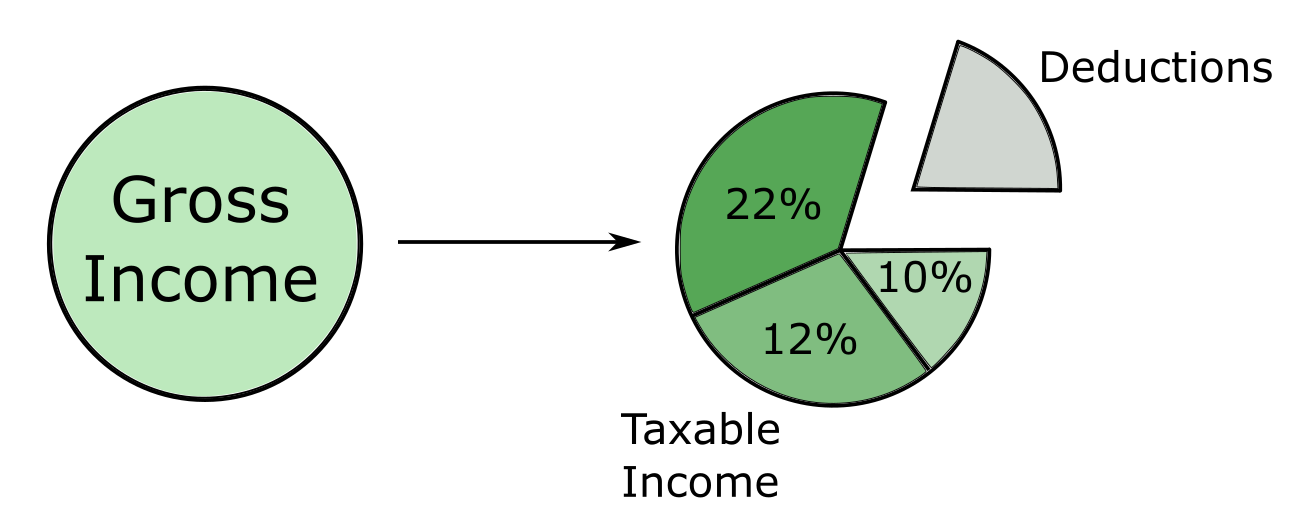
\includegraphics[width=0.6\textwidth]{TaxableIncomeIllustration}
\end{center}
\vfill
\pagebreak

Once the appropriate percentage of each segment has been accounted for, this forms the initial tax calculation, but then any applicable tax credits are subtracted, resulting in the final tax owed.
\begin{center}
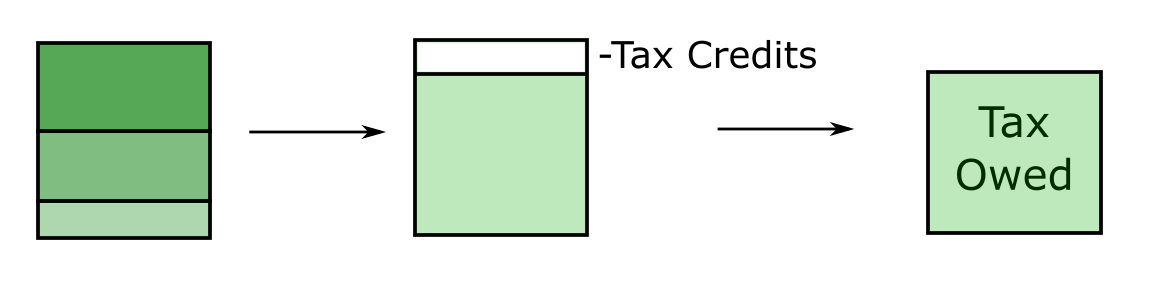
\includegraphics[width=0.6\textwidth]{TaxCreditIllustration}
\end{center}

For instance, if a taxpayer with a gross income of \$50,000 could claim deductions totaling \$13,000 and found \$500 worth of tax credits, it would work out something like this:
\begin{itemize}
\item \textbf{Gross Income:} \$50,000
\item \textbf{Taxable Income:} (subtract the deductions) \$50,000 - \$13,000 = \$37,000
\item \textbf{Initial Tax:} (skipping the calculation, but use the tax table) \$4242.50
\item \textbf{Final Tax Owed:} (subtract the credits) \$4242.50 - \$500 = \$3742.50
\end{itemize}
This person would owe a final tax bill of \$3742.50.\\

That's the basics of deductions and credits, but there's one final piece to the puzzle that we need to understand: \textbf{itemized} deductions vs. the \textbf{standard} deduction.

\begin{formula}{Standard and Itemized Deductions}
Taxpayers can choose to either take the standard deduction (listed on the tax table) or itemize their deductions (add up all the deductions that apply to them).\\

In practice, a taxpayer will add up the itemized deductions, and if this total is larger than the standard deduction, they will choose to go the itemized route.  If not, they will choose to use the standard deduction.
\end{formula}

Basically, there's a minimum deduction amount; if you find that your itemized deductions surpass that, you can use this larger sum as your deduction total.\\

With that, we're ready to work out a full example.
\begin{example}{Tax Calculation}
Use the 2020 tax table on page \pageref{Tax Table} to calculate the final tax owed by a single taxpayer whose details are given below.
\begin{center}
\begin{tabular}{r l}
Gross income: & \$65,000\\
Deductions: & \$3000: charitable donations\\
& \$6000: contribution to traditional IRA\\
& \$1500: education expenses\\
& \$300: cost of tax preparation\\
Tax credit: & \$500: energy-efficient appliances
\end{tabular}
\end{center}

\sol
First, decide whether this person will use itemized deductions or the standard deduction:
\begin{align*}
\marginnote{Calculate deductions}
\textrm{Itemized deductions } &= \$3000 + \$6000 + \$1500 + \$300\\
&= \$10,800
\end{align*}
Since the standard deduction for a single taxpayer (\$12,400) is larger, they will use the standard deduction.\\

Next, subtract the deductions from the gross income to find the taxable income:
\begin{align*}\marginnote{Find the taxable income}
\textrm{Taxable income } &= \textrm{ Gross income } - \textrm{ deductions (standard) }\\
&= \$65,000 - \$12,400\\
&= \$52,600
\end{align*}
\pagebreak

Now divide the taxable income into its brackets and calculate the tax owed from each bracket:
\begin{center}
\$52,600\marginnote{Divide the taxable income into brackets}

$\overbrace{
\begin{tabular}{r | c c c}
& & & \\
Dollars & 1 -- 9,875 & 9,876 -- 40,125 & 40,126 -- 52,600\\
%& & & \\
Tax Rate & 10\% & 12\% & 22\%\\
\end{tabular}
}$
\end{center}
\begin{align*}\marginnote{Multiply the amount in each bracket by that tax rate}
\textrm{Tax Owed } &= (9,875)(0.1) + (40,125-9,875)(0.12)\\ &\hspace{0.5in} + (52,600-40,125)(0.22)\\ &= \$7,362
\end{align*}

Finally, subtract the tax credit from this initial tax calculation to find the final amount that they owe:

\marginnote{Subtract the tax credit}\[\textrm{Final Tax Owed } = \$7,362 - \$500 = \boxed{\$6,872}\]
\end{example}

\begin{try}
Use the 2020 tax table to calculate the tax owed by a married couple filing jointly whose details are given below.
\begin{center}
\begin{tabular}{r l}
Gross income: & \$74,000\\
Deductions: & \$5500: charitable donations\\
& \$150: cost of tax preparation\\
Tax credit: & \$700: child tax credit
\end{tabular}
\end{center}
\end{try}

\checkoddpage
\ifoddpage{
\begin{adjustwidth}{0in}{-1.25in}
\begin{proc}{Tax Withholding}
During World War II, when the U.S. government was in dire need of tax revenue in order to avoid the rampant inflation that occurred during World War I, the IRS began to investigate tax withholding.  Rather than collecting taxes at the end of the year, they began to withhold taxes from workers' paychecks throughout the year, and then make up the difference at the end, either by a refund or an extra tax payment.  Milton Friedman, who won the 1976 Nobel Prize in economics, helped to formulate this plan.\\

New employees fill out a W-4 form, which is intended to calculate as accurately as possible how much they'll owe in taxes, so that the correct amount can be collected.  Many people like the idea of overestimating, because if more is withheld throughout the year, they receive a huge refund check.  However, this is not actually a good policy, since in effect they are giving the government an interest-free loan for the entire year with no strings attached.
\end{proc}
\end{adjustwidth}
} \else{
\begin{adjustwidth}{-1.25in}{0in}
\begin{proc}{Tax Withholding}
During World War II, when the U.S. government was in dire need of tax revenue in order to avoid the rampant inflation that occurred during World War I, the IRS began to investigate tax withholding.  Rather than collecting taxes at the end of the year, they began to withhold taxes from workers' paychecks throughout the year, and then make up the difference at the end, either by a refund or an extra tax payment.  It was Milton Friedman, who won the 1976 Nobel Prize in economics, who helped to formulate this plan.\\

New employees fill out a W-4 form, which is intended to calculate as accurately as possible how much they'll owe in taxes, so that the correct amount can be collected.  Many people like the idea of overestimating, because if more is withheld throughout the year, they receive a huge refund check.  However, this is not actually a good policy, since in effect they are giving the government an interest-free loan for the entire year with no strings attached.
\end{proc}
\end{adjustwidth}
} \fi